\documentclass[10pt,fleqn]{beamer}\usepackage[]{graphicx}\usepackage[]{color}
%% maxwidth is the original width if it is less than linewidth
%% otherwise use linewidth (to make sure the graphics do not exceed the margin)
\makeatletter
\def\maxwidth{ %
  \ifdim\Gin@nat@width>\linewidth
    \linewidth
  \else
    \Gin@nat@width
  \fi
}
\makeatother

\definecolor{fgcolor}{rgb}{0.345, 0.345, 0.345}
\newcommand{\hlnum}[1]{\textcolor[rgb]{0.686,0.059,0.569}{#1}}%
\newcommand{\hlstr}[1]{\textcolor[rgb]{0.192,0.494,0.8}{#1}}%
\newcommand{\hlcom}[1]{\textcolor[rgb]{0.678,0.584,0.686}{\textit{#1}}}%
\newcommand{\hlopt}[1]{\textcolor[rgb]{0,0,0}{#1}}%
\newcommand{\hlstd}[1]{\textcolor[rgb]{0.345,0.345,0.345}{#1}}%
\newcommand{\hlkwa}[1]{\textcolor[rgb]{0.161,0.373,0.58}{\textbf{#1}}}%
\newcommand{\hlkwb}[1]{\textcolor[rgb]{0.69,0.353,0.396}{#1}}%
\newcommand{\hlkwc}[1]{\textcolor[rgb]{0.333,0.667,0.333}{#1}}%
\newcommand{\hlkwd}[1]{\textcolor[rgb]{0.737,0.353,0.396}{\textbf{#1}}}%
\let\hlipl\hlkwb

\usepackage{framed}
\makeatletter
\newenvironment{kframe}{%
 \def\at@end@of@kframe{}%
 \ifinner\ifhmode%
  \def\at@end@of@kframe{\end{minipage}}%
  \begin{minipage}{\columnwidth}%
 \fi\fi%
 \def\FrameCommand##1{\hskip\@totalleftmargin \hskip-\fboxsep
 \colorbox{shadecolor}{##1}\hskip-\fboxsep
     % There is no \\@totalrightmargin, so:
     \hskip-\linewidth \hskip-\@totalleftmargin \hskip\columnwidth}%
 \MakeFramed {\advance\hsize-\width
   \@totalleftmargin\z@ \linewidth\hsize
   \@setminipage}}%
 {\par\unskip\endMakeFramed%
 \at@end@of@kframe}
\makeatother

\definecolor{shadecolor}{rgb}{.97, .97, .97}
\definecolor{messagecolor}{rgb}{0, 0, 0}
\definecolor{warningcolor}{rgb}{1, 0, 1}
\definecolor{errorcolor}{rgb}{1, 0, 0}
\newenvironment{knitrout}{}{} % an empty environment to be redefined in TeX

\usepackage{alltt}

\usepackage{lmodern}
\usepackage{knmiBeamer}
\usepackage{multirow}
\usepackage[skins]{tcolorbox}

\Engelstrue     % For English slides 
\renewcommand{\titleFigure}{figure/fogCover.jpg}

\usepackage{tikz}
\usepackage{verbatim}
\usetikzlibrary{arrows, shapes}

% ---------------
% Graphics folder
% ---------------
\graphicspath{{figure/}}

\title[Fog detection]{KNMI research on fog detection using cameras}
\subtitle{Meeting Port of Rotterdam}
\date{July 11, 2017}
\author[Pagani, Roth, Wauben]{Andrea Pagani, Martin Roth\\ and Wiel Wauben}
%\author[M. Roth (\MYhref{mailto:roth@knmi.nl}{roth@knmi.nl})]{Martin Roth\texorpdfstring{\\[2mm] \scriptsize \href{mailto:roth@knmi.nl}{roth@knmi.nl}\\[4mm] {\scriptsize Joint work with A. Buishand and G. Jongbloed}}{}}
\IfFileExists{upquote.sty}{\usepackage{upquote}}{}
\begin{document}
\tikzstyle{every picture}+=[remember picture]




\begin{frame}
 \titlepage
\end{frame}

 \begin{frame}{Outline}
  \begin{itemize}
   \item Motivation for reseach on fog
   \item Current project purpose, scope, benefits
   \item Project highlights
   \item Machine Learning example
   \item Challenges
   \item Tools used
   \item Q\&A
 \end{itemize}
 \end{frame}




\begin{frame}{Fog as hazard}
 \begin{textblock*}{5cm}(7.4cm,2.4cm)
  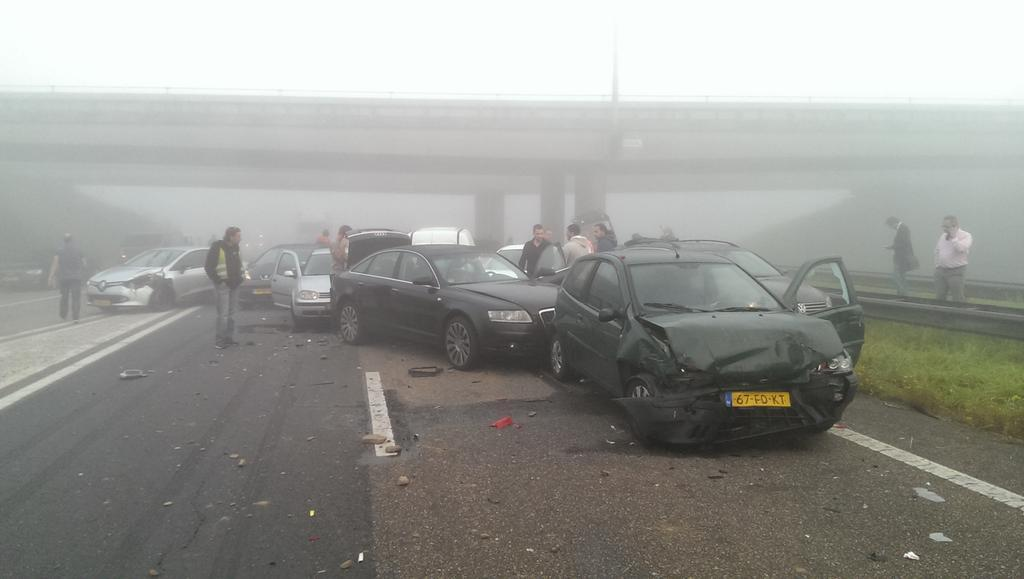
\includegraphics[width=5cm]{Accident.jpeg}
 \end{textblock*}
 \begin{textblock*}{5cm}(7.4cm,5.5cm)
  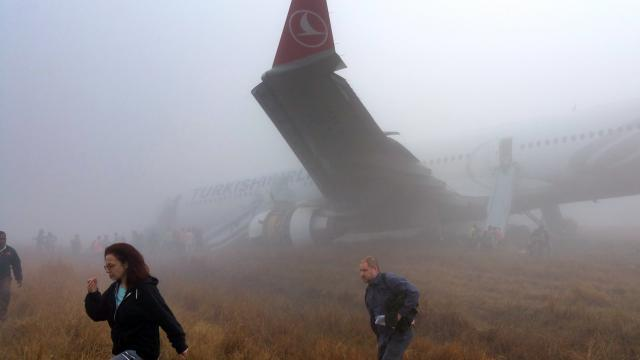
\includegraphics[width=5cm]{airplane.jpg}
 \end{textblock*}
\begin{itemize}
  \item Substantial impact on air,\\ marine, and road traffic
  \item Loss of life comparable to that of\\ tornadoes or even winter storms\footnote{Gultepe, I. et al. (2007): Fog research: A review of past achievements and future perspectives. \emph{Pure and Applied Geophysics}, \textbf{164}, 1121--1159.}
  \item May form and dissipate suddenly
  \item Often only a local phenomenon
  \item Not easy to accurately forecast
  \item Satellites are not pointing to NL 24/7
 \end{itemize}
\end{frame}

\begin{frame}{KNMI DataLab project: Purpose, Scope, Benefits}
\begin{itemize}
\item \textbf{Purpose:} use cameras to identify fog conditions to issue safety hazards
\item \textbf{Scope:} daylight fog detection from static cameras using image analysis
\item \textbf{Benefits:}
\begin{itemize}
\item \textit{Society: }
\begin{itemize}
\item human lives
\item economic
\end{itemize}
\item \textit{KNMI:}
\begin{itemize}
\item better widespread observations of fog conditions
\item feed the fog observations in KNMI models (re-analysis) $\Rightarrow$ better fog modeling/predictions
\end{itemize}
\end{itemize}

\end{itemize}
\end{frame}

\begin{frame}{Example: availability of sensors and traffic cameras}
 \begin{textblock*}{5cm}(1.2cm,3.0cm)
  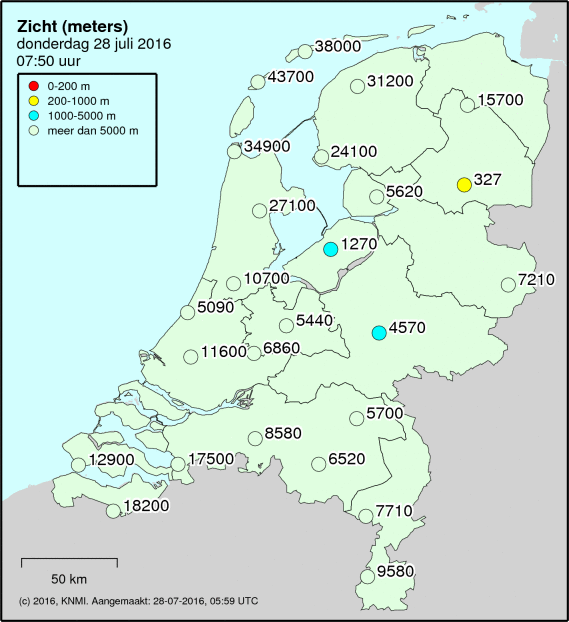
\includegraphics[width=5cm]{SensorPlacement.png}
 \end{textblock*}
 \begin{textblock*}{5cm}(7.0cm,3.7cm)
  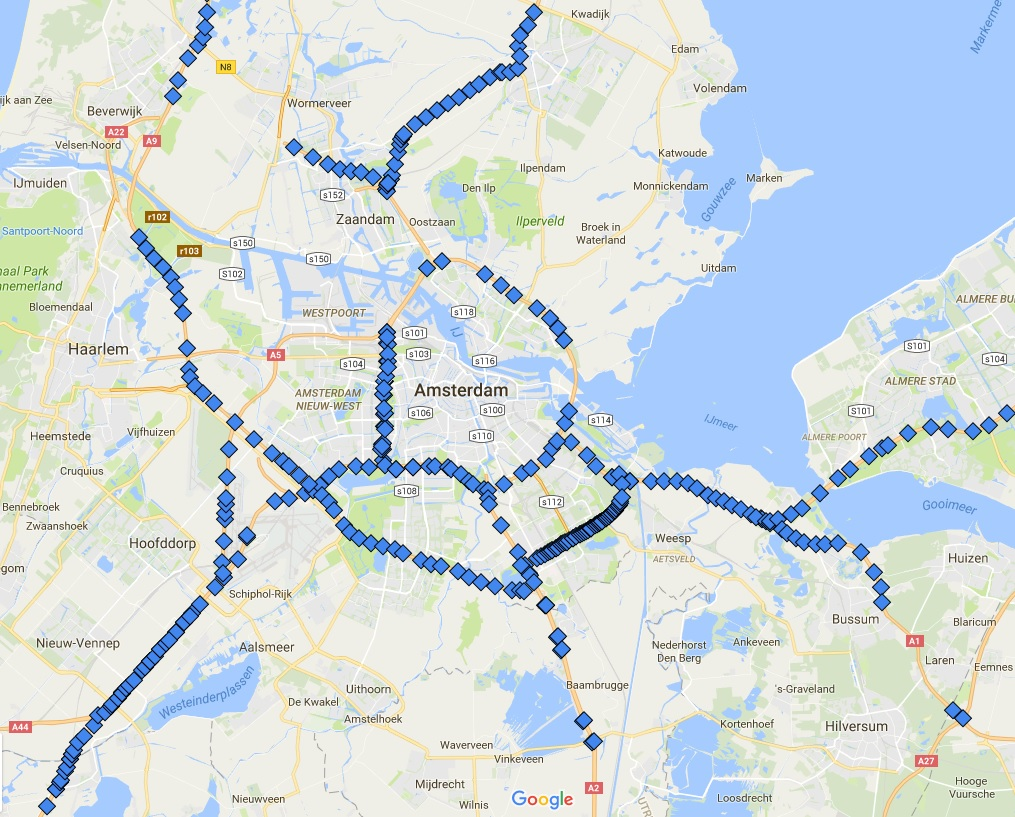
\includegraphics[width=5cm]{CameraPlacement.jpg}
 \end{textblock*}
\end{frame}









%Present a slide with the status and progress of the project  (e.g. list successes and obstacles).
\begin{frame}{Project status}
\begin{itemize}
\item \textbf{Successes:}
\begin{itemize}
\item{ Analyzed images of 1.5 years De Bilt - good results}
\item {Analyzed images of 1.5 years Twente - so and so results}
\item {Built an archive for images at KNMI Cabauw station and Scotland Traffic (since October 2016)}
\item {Built an archive for images from 160 RWS highway location (since June 2017)}
\item {Successful interaction RWS: collaboration project (end 2016 - full 2017)}

\end{itemize}

\item \textbf{Obstacles:}
\begin{itemize}
\item{Access to camera images: privacy issues}
\item{More data needed to thoroughly test algorithms}
\item{Co-location of cameras and visibility sensors for evaluation}
\item{Generalization from one scene to another is hard}
%\item{Limited time for the project by the PIs}
\end{itemize}
\end{itemize}
\end{frame}



\begin{frame}{Machine learning approach}
\vspace*{-5mm}
Example elaboration and feature: edge detection
\begin{knitrout}
\definecolor{shadecolor}{rgb}{0.969, 0.969, 0.969}\color{fgcolor}
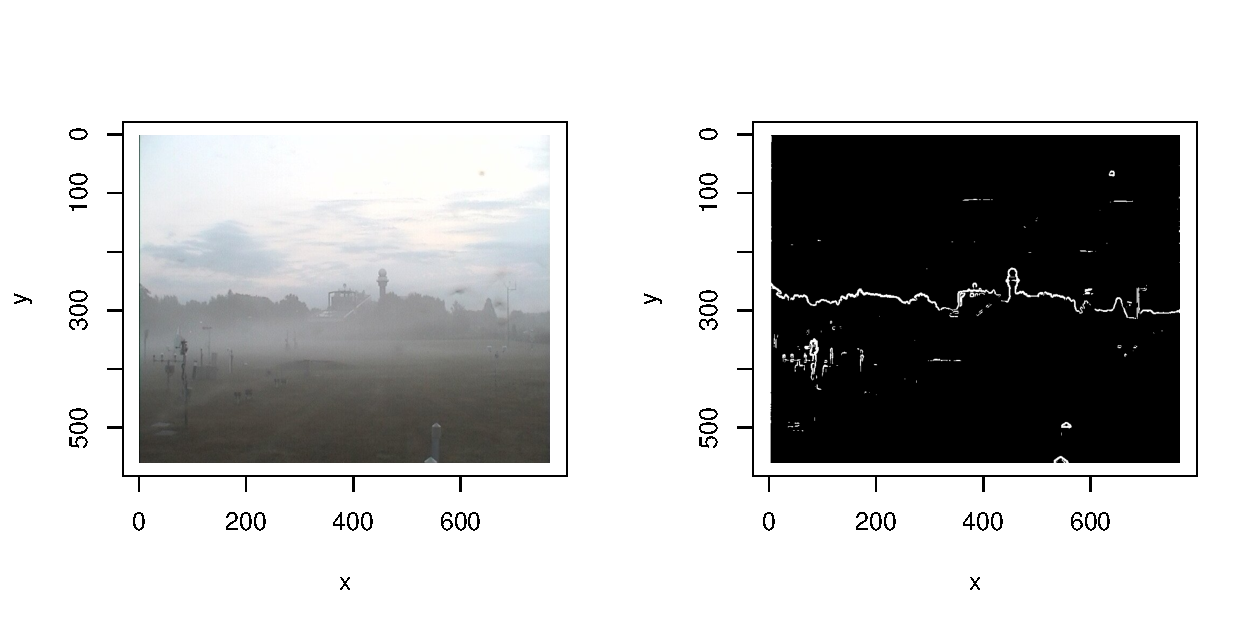
\includegraphics[width=\maxwidth]{figure/LandmarkPlotClear-1} 

\end{knitrout}
 \begin{textblock*}{10cm}(1.5cm,8cm)
  Consider the mean number of edges in the picture as feature.
 \end{textblock*}
\end{frame}







\begin{frame}{Machine Learning: De Bilt classification tree} 
\scriptsize{keys for reading a node:\\
 fraction of fog cases in the node/sub-tree\\
 \# of cases  \textemdash \% of total cases}
 

\begin{knitrout}
\definecolor{shadecolor}{rgb}{0.969, 0.969, 0.969}\color{fgcolor}
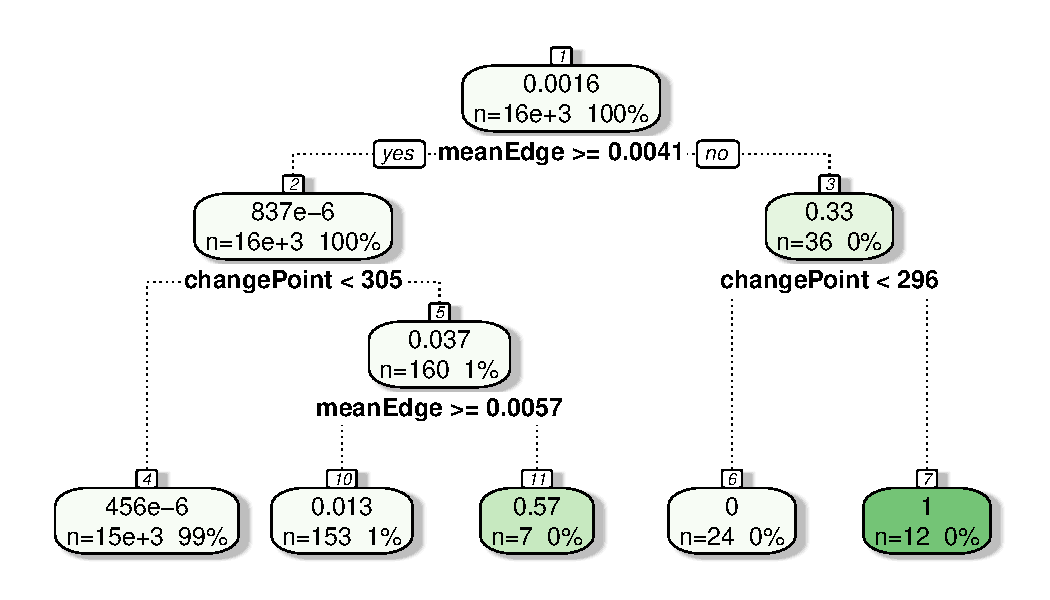
\includegraphics[width=\maxwidth]{figure/ClassificationTree-1} 

\end{knitrout}
% keys for reading a node:
% fraction of fog cases in the node/sub-tree
% # of cases
% \% of total cases
\end{frame}


%%%%%%%%%%%%%%%%%%%%%%%%%%%%%%%MODIFIED ANDREA%%%%%%%%%%%%%%%%%%%%%%%%%%%%%%%%%%%%%%%%%%%%%%%%%%%%%%%%%%%%%%%

\begin{frame}{Challenges: example Twente KNMI station}\centering
%The situation in Twente is different for two reasons, the wide angle of the
%camera makes the horizontal averaging of the transmission rate less appropriate.
%Moreover, even on a clear day there are only a few edges in the image (which are
%mostly very close to the camera, i.e. from the equipment of the automatic 
%weather station). Nevertheless, it was quite simple to detect failures of the 
%visibility sensor using the two described features, such as during the afternoon
%of August 23 2015, where the sensor consistently gave $MOR < 250$, although the 
%image is very clear.
 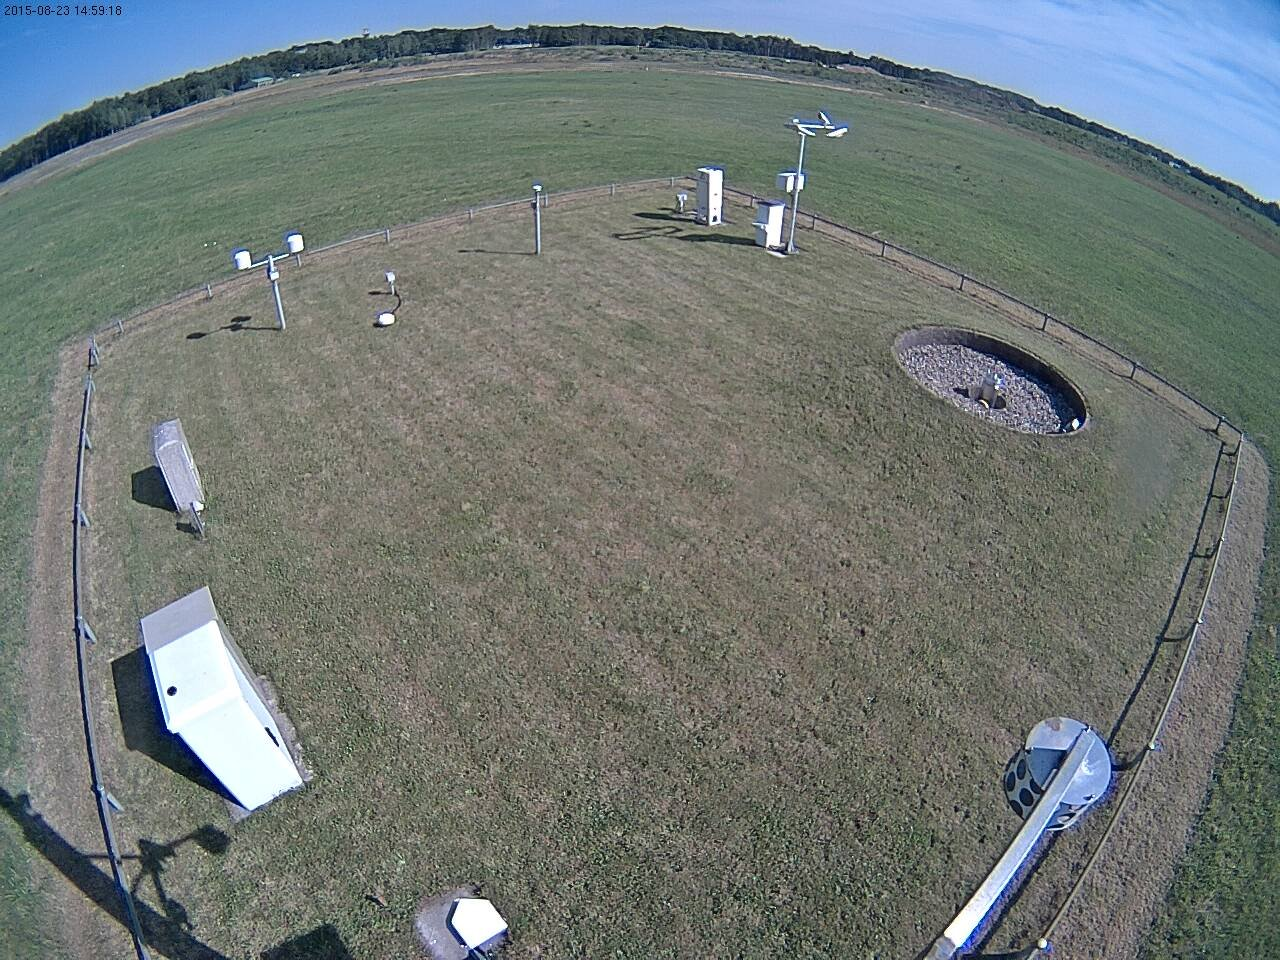
\includegraphics[width=5cm]{EHTW_201508231400.jpg}
 \begin{itemize}
  \item fish-eye lens
  \item only a few edges in the range of 50--250\,m
  \item fully unprotected camera
 \end{itemize}
\end{frame}




\begin{frame}{Examples: weather (un)protection}%\centering
\begin{columns}
\column{0.2\textwidth}
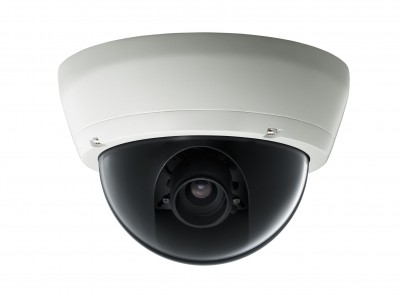
\includegraphics[height=2cm]{figure/wideCamera}

\column{0.8\textwidth}
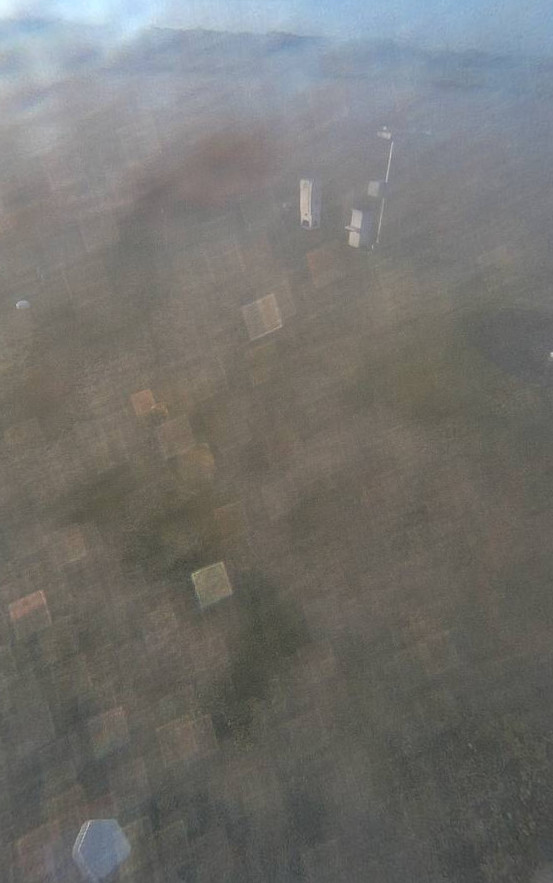
\includegraphics[height=3cm]{inst/extdata/cornerCasesTwente/EHTW_201506280400.jpg} \\
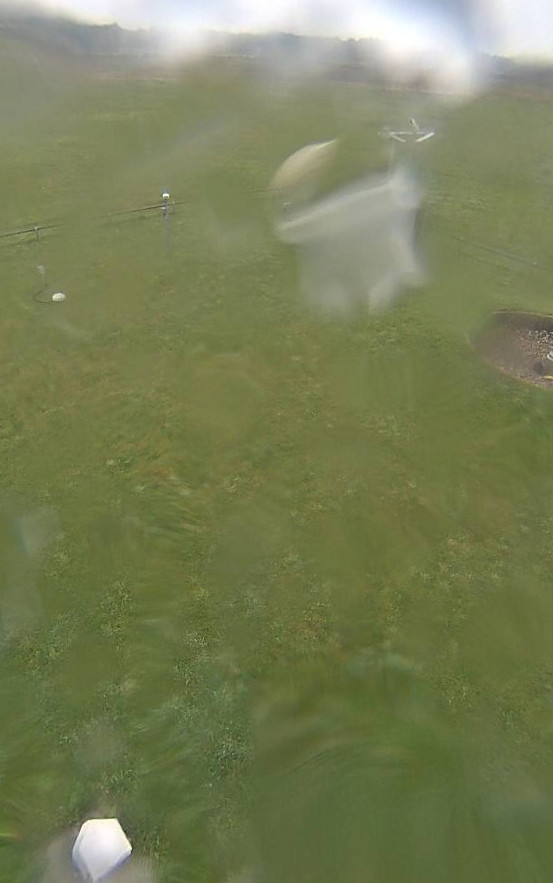
\includegraphics[height=3cm]{inst/extdata/cornerCasesTwente/EHTW_201510060700.jpg} \\

\end{columns}
\begin{textblock*}{5cm}(6.2cm,3.85cm)
Ice on the camera enclosure\\
\vspace{2.7cm}
Water drops on the camera enclosure
\end{textblock*}



\end{frame}
















%%%%%%%%%%%%%%%%%%%%%%%%%%%%%%%MODIFIED ANDREA END%%%%%%%%%%%%%%%%%%%%%%%%%%%%%%%%%%%%%%%%%%%%%%%%%%%%%%%%%%%%%%%




\begin{frame}{Tools and technologies used}

\begin{columns}
\column{0.65\textwidth}
\begin{itemize}
\item{Maturing more knowledge and confidence in ML techniques}
\item{Confluence project repository}
\item{Project/task management: Trello}
\item{Heavy use of parallel computation in R}
\item{Parallel cluster on clouds providers}
\item{GitHub repository for versioning}
\item{Storage of the image features and metadata in postgreSQL}
% \begin{itemize}
% \item{Open source nonSQL DB technology}
% \item{Based on the heritage of Google BigTable}
% \item{Horizontal scaling to handle billions of rows}
% \end{itemize}
\end{itemize}

\column{0.45\textwidth}
%\hspace{2cm}

\includegraphics[height=2cm]{figure/R_logo}\\
\vspace{0.5cm}

\includegraphics[width=4cm]{figure/aws}\\
%\vspace{0.1cm}
\end{columns}


\begin{textblock*}{2cm}(10.7cm,4.5cm)

\includegraphics[width=2cm]{figure/postgresql_logo}
\end{textblock*}


\begin{textblock*}{2cm}(10.2cm,2cm)
 
\includegraphics[width=2cm]{figure/Git_logo}
\end{textblock*}

\begin{textblock*}{2cm}(10.5cm,3.5cm)
 
\includegraphics[width=2cm]{figure/trello}
\end{textblock*}


\end{frame}



\begin{frame}{Questions to Port of Rotterdam}
 \begin{itemize}
\item{What is Port of Rotterdam using for fog detection?}
\item{Has port of Rotterdam a CCTV network? More than \scriptsize{\url{https://www.portofrotterdam.com/nl/de-haven/webcams}} ?}
\item{Interested in a camera-based fog estimation?}
\item{Possibility for KNMI to access camera picture for research purposes?}
\item{Does Port of Rotterdam have a picture/video archive?}
\item{Are metedata available (e.g., location, direction, resolution, FOV, settings)?}
\end{itemize}
\end{frame}















% \begin{frame}{Validation plot}
% Focusing on prominent regions in the plot, we could also identify several cases
% where there is clearly an adaptation of the camera taking place and that
% sometimes the different scenery is not only present for one picture but for an
% extended period of time.
% 
% The next plot shows the modelled log(MOR) for the validation set. The 


% \end{frame}



% \begin{frame}{Next steps}
% 
%  \begin{block}{More testing \alert{$\Rightarrow$} need more representative images}
%  \end{block}
%  
%  \begin{block}{More research into features and different ML algorithms}
%  \end{block}
%  
%  \begin{block}{Use multiple cameras (spatio-temporal model)}
%  \end{block}
%  
%  % \begin{block}{Next directions}
%  % \begin{itemize}
%  %  \item use additional features, e.g. wind or dew point temperature
%  %  \item use clustering for unsupervised learning
%  % \end{itemize}
%  % \end{block}
% \end{frame}

\appendix



\begin{frame}{Back-up slides}
\end{frame}

\begin{frame}{Features extracted from images}


\begin{itemize}
\begin{footnotesize}
\item{Mean Edges: for finding the boundaries of objects within images. It works by detecting discontinuities in the image (e.g., foreground and background elements).}
\item{Mean Brightness: perception of a source of radiating/reflecting light.}
\item{Mean Saturation: is a measure of the purity of the color. The purest (most saturated) color is achieved by using just one wavelength, less pure come from a combination at different wavelengths.}
\item{Mean HUE: perception of a source of being similar to one of the perceived colors: red, yellow, green, and blue, or to a combination of two of them.}
\item{Fractal Dimension: self similarity in filling space.}
\item{Transmission smoothness: transmission of the darkchannel of the image (smoothed indicator).}
\item{Transmission changepoint: horizontal point where the transmission of the dark channel is subject to change.}
\end{footnotesize}
\end{itemize}





\end{frame}





\begin{frame}{Contingency Table image features only}\centering
% 
\begin{itemize}
\item {Picture-only features test set (8 months of observations)}

% 
\end{itemize}
\begin{table}
    %\setlength{\extrarowheight}{2pt}
    \begin{tabular}{cc|c|c|}
       & \multicolumn{1}{c}{} & \multicolumn{2}{c}{Reference}\\
       & \multicolumn{1}{c}{} & \multicolumn{1}{c}{FALSE}  & \multicolumn{1}{c}{TRUE} \\\cline{3-4}
       \multirow{2}*{Prediction}  & FALSE & 15736  & 34 \\\cline{3-4}
      & TRUE & 38 &6 \\\cline{3-4}
    \end{tabular}
  \end{table}
  
  \begin{itemize}
\item {Issues mentioned above play a role in the false positive/negative}
\item{POD: 0.1500000}
\item{FAR: 0.002409028}

% 
\end{itemize}
  
% % Original
% % ##
% % ## Reference
% % ## Prediction FALSE TRUE
% % ## FALSE 15736 34
% % ## TRUE 38 6
% 
% 
 \end{frame}

\begin{frame}{Contingency Table with meteo features}\centering
% 
\begin{itemize}
\item {Picture and meteo features test set (8 months of observations)}
\item{Filtered out continuous rain conditions and wind speed $\geq$ 3.5 m/s}
% 
\end{itemize}
\begin{table}
    %\setlength{\extrarowheight}{2pt}
    \begin{tabular}{cc|c|c|}
       & \multicolumn{1}{c}{} & \multicolumn{2}{c}{Reference}\\
       & \multicolumn{1}{c}{} & \multicolumn{1}{c}{FALSE}  & \multicolumn{1}{c}{TRUE} \\\cline{3-4}
       \multirow{2}*{Prediction}  & FALSE & 6743  & 14 \\\cline{3-4}
      & TRUE & 165 & 26 \\\cline{3-4}
    \end{tabular}
  \end{table}
  
  \begin{itemize}
\item {Meteorological features are not selected except air temperature}
\item{POD: 0.6500000}
\item{FAR: 0.02388535}


% 
\end{itemize}
 
 \end{frame}



\end{document}
